\documentclass[10pt]{article}
\usepackage{amsmath} 
\usepackage{graphicx}

\begin{document}

\textbf{Problema 1: Campo medio}
\\

\begin{equation}
H = -J_2 \sum_{\langle i,j\rangle} \sigma_i \sigma_j - J_4 \sum_I \sigma_{I1}\sigma_{I2}\sigma_{I3}\sigma_{I4}
\end{equation}

Hamiltoniano de prueba:

\begin{equation}
H_0 = -\eta \sum_i \sigma_i
\end{equation}

Desigualdad de Bogoliuvob-Peierls:

\begin{equation}
f \leq f_{\rho} = f_0 + \dfrac{1}{N} \langle H - H_0 \rangle_0.
\end{equation}

Funci\'on de partici\'on para el hamiltoniano de prueba:

\begin{align}
\mathcal{Z}_0 &= \sum_{\lbrace s_i\rbrace} e^{-\beta H_0} \nonumber \\
&= \sum_{\lbrace s_i\rbrace} \exp \left[ \beta \eta \sum_i s_i  \right] \nonumber \\
&= \sum_{\lbrace s_i\rbrace} \prod_i  e^{\beta \eta s_i} \nonumber \\
&= \prod_i \sum_{s_i=\pm1} e^{\beta \eta s_i}  \nonumber \\
&= \left[ e^{-\beta \eta} + e^{\beta \eta} \right]^N \nonumber \\
&= \left[ 2 \cosh\left(\beta \eta\right) \right]^N, \nonumber \\
&= \mathcal{Z}_{01}^N,
\end{align}

donde 

\begin{equation}
\mathcal{Z}_{01} = 2 \cosh\left(\beta \eta\right).
\end{equation}

Energ\'ia libre:

\begin{align}
f_0 &= -\dfrac{1}{\beta N} \ln \mathcal{Z}_0 \nonumber \\
&= -\dfrac{1}{\beta} \ln \left[ 2 \cosh\left(\beta \eta\right) \right]
\end{align}

Magnetizaci\'on:

\begin{align} \label{eq:BC_m0}
m_0 &= \langle s_i \rangle_0 \nonumber \\
&= \dfrac{1}{\mathcal{Z}_{01}} \sum_{s_i=\pm1} s_i e^{\beta \eta s_i} \nonumber \\
&= \dfrac{1}{\mathcal{Z}_{01}} \left[-e^{-\beta \eta} + e^{\beta \eta} \right] \nonumber \\
&= \tanh\left( \beta \eta \right)
\end{align}


Valores medios de los hamiltonianos respecto del hamiltoniano de prueba:

\begin{align}
\langle H_0 \rangle_0 &= -\eta \sum_i \langle s_i \rangle_0  \nonumber \\
&= -\eta N m_0 
\end{align}

\begin{align}
\langle H \rangle_0 &= -J_2 \sum_{\langle i,j\rangle} \langle s_i s_j \rangle_0 - J_4 \sum_I \langle\sigma_{I1}\sigma_{I2}\sigma_{I3}\sigma_{I4} \rangle_0 \nonumber \\
&= -J_2 \sum_{\langle i,j\rangle} \langle s_i\rangle_0^4 - J_4 \sum_I \langle\sigma_{I1}\rangle_0^4  \nonumber \\
&= -2 J_2 N m_0^2 - J_4 N m_0^4 \nonumber
\end{align}

Proponemos la funci\'on variacional 

\begin{align} \label{eq:BC_Phi}
\Phi(\eta) &= f_0 + \dfrac{1}{N} \langle H - H_0 \rangle_0 \nonumber \\
&= -\dfrac{1}{\beta} \ln \left[2 \cosh\left(\beta \eta\right) \right] -2 J_2 m_0^2 - J_4 m_0^4 + \eta m_0
\end{align}

Derivamos con respecto a $\eta$ e igualamos a cero para hallar el m\'inimo

\begin{align}
\dfrac{\partial \Phi}{\partial \eta} &= - \tanh\left(\beta \eta\right) - 4 J_2 m_0 \dfrac{\partial m_0}{\partial \eta} - 4 J_4 m_0^3 \dfrac{\partial m_0}{\partial \eta} + m_0 + \eta \dfrac{\partial m_0}{\partial \eta} \nonumber \\
&= \left(\eta - 4 J_2 m_0 - 4 J_4 m_0^3\right) \dfrac{\partial m_0}{\partial \eta},
\end{align}

donde usamos la igualdad \ref{eq:BC_m0}.

La expresi\'on anterior implica que la soluci\'on al problema variacional es 

\begin{equation}\label{eq:eta}
\eta = 4 J_2 m_0 + 4 J_4 m_0^3.
\end{equation}

Reemplazando el valor de $\eta$ en \ref{eq:BC_m0},

\begin{equation}
m_0 = \tanh\left[\beta (4 J_2 m_0 + 4 J_4 m_0^3)\right].
\end{equation}

Definimos las variables $\tilde{\beta} \equiv 4 J_2 \beta$ y $J \equiv J_4/J_2$. De este modo, la ecuaci\'on anterior queda

\begin{equation}
m_0 = \tanh\left[\tilde{\beta} (m_0 + J m_0^3)\right].
\end{equation}

La energ\'ia libre est\'a dada por la expresi\'on que minimiza la funci\'on $\Phi(\eta)$ con respecto a $\eta$. Es decir,

\begin{equation}
f_{\mathrm{mf}}(T,B) = \min_{\eta} \Phi(\eta).
\end{equation}

Utilizando \ref{eq:eta} y \ref{eq:BC_Phi}, tenemos

\begin{equation}
f_{\mathrm{mf}}(T,B=0) = -\dfrac{1}{\beta} \ln \left[2 \cosh\left(\beta ( 4 J_2 m_0 + 4 J_4 m_0^3)\right) \right] +2 J_2 m_0^2 + 3 J_4 m_0^4.
\end{equation}

Reescalamos la energ\'ia en unidades de $J_2$, definiendo $\tilde{f}_{\mathrm{mf}} \equiv f_{\mathrm{mf}}/J_2$. As\'i obtenemos

\begin{equation}
\tilde{f}_{\mathrm{mf}}(T,B=0) = -4\tilde{\beta}^{-1} \ln \left[2 \cosh\left(\tilde{\beta} ( m_0 + J m_0^3)\right) \right] +2 m_0^2 + 3 J m_0^4.
\end{equation}

Haciendo un desarrollo de Taylor a orden 6,

\begin{align}
\tilde{f}_{\mathrm{mf}}(T,B=0) =& \;C + 2(1-\tilde{\beta}) m_0^2 + 
\left(3J - 4J\tilde{\beta} + \dfrac{\tilde{\beta}^3}{3} \right) m_0^4 \nonumber \\
&+ \left(-2 J^2\tilde{\beta} + \dfrac{4J\tilde{\beta}^3}{3} - \dfrac{4\tilde{\beta}^5}{45}\right) m_0^6 + \mathcal{O}(m_0^8)
\end{align}

donde $C = -4\ln(2)/\tilde{\beta}$ es un t\'ermino aditivo que resulta irrelevante. Vemos entonces que la energ\'ia libre queda expresada en forma de funci\'on de Landau

\begin{align}
\tilde{f}_{\mathrm{mf}}(T,B=0) = C + \dfrac{a_2}{2} m_0^2 + 
\dfrac{a_4}{4} m_0^4 + \dfrac{a_6}{6} m_0^6 + \mathcal{O}(m_0^8),
\end{align}

con coeficientes 

\begin{align*}
a_2(T,J) &= 4 (1-\tilde{\beta})\\
a_4(T,J) &= 4\left( 3J - 4J\tilde{\beta} + \dfrac{\tilde{\beta}^3}{3} \right) \\
a_6(T,J) &= 6 \left(-2 J^2\tilde{\beta} + \dfrac{4J\tilde{\beta}^3}{3} - \dfrac{4\tilde{\beta}^5}{45}\right)
\end{align*}

Para construir el diagrama de fases, comencemos analizando si existe transici\'on de segundo orden. La l\'inea de segundo orden se obtiene cuando $a_2=0$ y $a_4>0$. De la primera condici\'on, obtenemos que $\tilde{\beta}_c = 1$, mientras que de la segunda,


\begin{equation}
J < \dfrac{\tilde{\beta}_c^3}{3(4\tilde{\beta}_c-3)}=\dfrac{1}{3}.
\end{equation}

De la definici\'on de $\tilde{\beta}$, se deduce que $k_B T/J_2 = 4 /\tilde{\beta}$, por lo que la temperatura cr\'itica satisface $k_B T_c/J_2 = 4$.

\begin{figure}
\centering
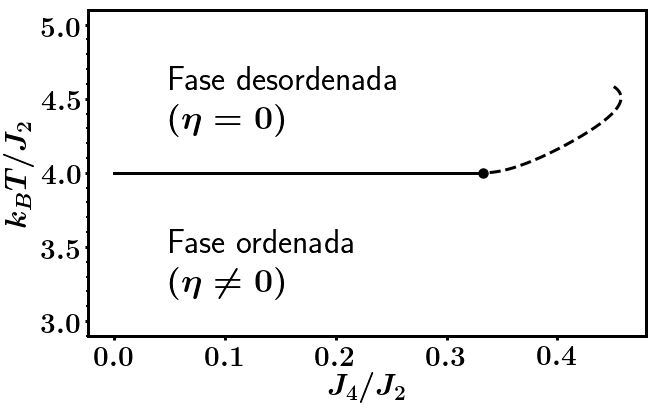
\includegraphics[scale=0.5]{phase_diagram.png}
\caption{Diagrama de fases.}
\end{figure}


\end{document}
